\chapter{Визуальные языки и их свойства}
\label{chapter1}

В этой главе приводится контекст работы и основные понятия, используемые в 
дальнейшем при изложении результатов диссертации. 

\section{Визуальное моделирование}
Идея использовать чертежи для разработки сложных систем родилась из аналогии с 
инженерными дисциплинами --- так же как, например, при строительстве дома проект 
разрабатывается архитектором, а потом реализуется строителями, хотелось бы иметь 
возможность подготовить проект программной системы, а затем, когда все 
архитектурные решения уже приняты, просто его реализовать. Это позволило бы 
добиться разделения труда как в инженерных дисциплинах --- отделить 
проектирование от реализации, осуществлять эту деятельность людьми с разными 
навыками и разным уровнем подготовки, и тем самым добиться удешевления разработки 
ПО и повышения его качества. Естественно по аналогии с инженерными дисциплинами 
использовать для описания архитектуры системы графические чертежи.

Однако разработка программных систем имеет ряд особенностей, делающих прямое 
заимствование опыта из инженерных дисциплин невозможным. Программное обеспечение 
незримо, поэтому изображать его можно по-разному, каждый человек может по-своему 
представлять себе программу. Это существенно отличает проектирование ПО от 
проектирования объектов реального мира --- архитектор рисует чертёж здания, 
который напоминает вид этого здания, когда оно будет достроено. Программа, 
именно как сама программа, не выглядит никак --- мы имеем дело лишь с её кодом, 
или с её пользовательским интерфейсом, или с внешними проявлениями её работы. 
Поэтому "`чертёж"' ПО --- это всегда некоторая договорённость между 
разработчиками о том, что и как будет изображено на "`чертеже"'. Такая договорённость называется 
%TODO: кто, когда и как ввёл
\textit{метафорой визуализации}. Например, при использовании 
языка UML для визуализации архитектуры системы мы договариваемся, что классы 
изображаются в виде прямоугольников, а случаи использования --- в виде овалов. 
Поскольку язык UML является де-факто стандартом индустрии и очень широко 
распространён, то нарисованная одним разработчиком схема будет скорее всего 
правильно понята другими разработчиками. Бывают и менее распространённые 
визуальные языки, каждый из которых тоже использует какие-то графические символы 
для изображения сущностей моделируемой системы.

Поскольку программа не имеет какого-то внешнего вида и для её визуализации 
используются метафоры, то оказывается невозможным нарисовать 
"`программу целиком"', каждая визуальная модель описывает какой-то свой аспект 
системы. При этом, даже если изображаемый аспект системы фиксирован, изображать 
его можно по-разному, используя разные уровни детализации или отображая на 
диаграммах разную информацию. Например, если мы хотим изобразить архитектуру 
системы с помощью языка UML, мы в зависимости от ситуации можем сделать это с 
помощью диаграмм компонентов или диаграмм классов, причём, если мы рисуем 
диаграммы для заказчика или начальства, они должны содержать меньше технических 
подробностей, чем диаграммы для программистов. Таким образом, каждая диаграмма 
рисуется с какой-то определённой целью для какой-то определённой категории 
людей, при этом изображая какой-то определённый аспект системы. Поэтому выделяют 
понятие "`\textit{точка зрения моделирования}"'
%TODO: кто, когда и как ввёл
, в которое входят все перечисленные выше 
соображения о назначении диаграммы. Понятие точки зрения моделирования применимо 
не только к конкретной диаграмме, но и к языку моделирования в целом, поэтому 
весьма важно для дальнейшего изложения. Каждый язык предназначен для рисования 
диаграмм, описывающих систему с точки зрения, свойственной этому языку. 
Поэтому это понятие можно с одной стороны использовать как базис классификации 
языков, с другой стороны, как мотивировку для создания новых языков. Здесь 
следует отметить, что язык UML здесь рассматривается как набор взаимосвязанных 
языков, а не как один язык.

Следующее вводимое здесь понятие тесно связано с точками зрения моделирования 
--- \textit{семантический разрыв}
%TODO: кто, когда и как ввёл
. Визуальная модель не может содержать в себе всю 
информацию о системе, потому что модель --- это всегда упрощение моделируемого 
объекта. Таким образом, модель системы, как правило, не содержит в себе всей 
информации, необходимой для генерации или интерпретации программы, описываемой 
этой моделью. То есть, среди точек зрения моделирования не бывает точки зрения 
исполнителя. Тот факт, что любая модель системы принципиально содержит 
недостаточно информации для исполнителя, и называется семантическим разрывом ---
разрывом между семантикой модели и семантикой исполняемой программы. 
Семантический разрыв делает невозможной полную генерацию кода программы по 
визуальной модели, либо заставляет вносить в модель столько информации, что 
она становится столь же сложна, что и моделируемая программа. Поэтому очень 
многие диаграммы на языке UML рисуются только как иллюстрации к технической 
документации, и основной объём работы по реализации системы вне зависимости от 
наличия визуальных моделей приходится выполнять программистам. Такая ситуация 
нежелательна, поскольку хотелось бы более продуктивно переиспользовать труд 
проектировщиков. Поэтому семантический разрыв пытаются преодолеть.

Существует класс инструментов, поддерживающих визуальное моделирование. 
Такие инструменты по традиции называют \textit{CASE-системами} (или \textit{CASE-пакетами}), 
хотя этот термин весьма неточен. Исторически термин "`CASE"' 
%TODO: кто, когда и как ввёл
(Computer-Aided Software Engineering) обозначал применение методов и 
технологических средств для разработки программного обеспечения с помощью 
компьютера, то есть обычные текстовые среды разработки с точки зрения такого 
определения --- тоже CASE-инструменты. В таком значении этот термин давно 
%TODO: почему?
не используется, сейчас CASE относится прежде всего к средствам разработки 
программного обеспечения, использующим визуальные модели. CASE-системы могут 
покрывать как весь цикл разработки программного обеспечения, так и отдельные 
его этапы. Для обозначения первой категории CASE-систем используется термин 
\textit{I-CASE}
%TODO: кто, когда и как ввёл
(\textit{Integrated CASE}), такие системы имеют тенденцию включать в себя всё 
необходимое для разработки ПО, от средств анализа требований до средств 
автоматизации тестирования и средств управления проектом, при этом интегрируются 
с компиляторами, отладчиками, профилировщиками и другими требуемыми для 
разработки инструментами. Средства из второй категории традиционно подразделяют 
на средства поддержки первых этапов водопадной модели жизненного цикла ПО 
(анализа и проектирования), называемые \textit{Upper CASE}
%TODO: кто, когда и как ввёл
, и нижних этапов этой модели 
(реализации и тестирования), называемые \textit{Lower CASE}
%TODO: кто, когда и как ввёл
. Исторически первые CASE-системы (например, PSL/PSA~\cite{teichroew1977psl}) относились к категории Upper CASE, поскольку 
автоматизировали исключительно анализ требований, затем 
(в 80-х и начале 90-х годов 20-го века) широкое распространение получили 
I-CASE-средства. Связано это с тем, что в те времена основной объём 
разрабатываемых программных продуктов приходился на программное обеспечение для 
мэйнфреймов, автоматизирующее бизнес-процессы крупных компаний. Там 
CASE-средства играли роль интегрированных средств разработки, в которых 
писалось всё программное обеспечение целиком, и они интегрировались со всеми 
остальными необходимыми средствами разработки, доступными для нужной платформы. 
Наиболее популярные современные CASE-средства, как правило, ориентированы на 
автоматизацию этапов анализа и проектирования, таким образом, относятся к 
Upper CASE по данной классификации.

Современные CASE-системы, как правило, состоят из большого числа компонентов. 
Наиболее важный из них --- репозиторий, база данных, хранящая в себе всю 
информацию о разрабатываемой системе, с репозиторием работают все остальные 
компоненты. Вводится информация в репозиторий посредством редакторов, которые 
могут быть визуальными редакторами диаграмм, текстовыми редакторами, редакторами 
таблиц и т.д. Впоследствии репозиторий могут использовать генераторы, которые по 
модели системы генерируют код на текстовых языках (как правило, фрагменты 
программы, например, объявления классов без реализаций) или документацию, 
валидаторы, проверяющие корректность, целостность и полноту содержимого 
репозитория, интерпретаторы и отладчики, использующие хранящуюся в репозитории 
модель системы для непосредственного исполнения. Кроме того, в состав 
CASE-систем могут входить вспомогательные средства, такие как текстовый редактор 
(для работы со сгенерированным кодом или документацией), редактор экранных форм, 
средства управления проектом, средства интеграции с системами контроля версий, 
средства импорта и экспорта моделей, и т.д.

\section{Структура визуальных языков}
Визуальные языки могут применяться и без какой-либо инструментальной поддержки, 
например, для рисования набросков архитектуры системы, моделей предметной 
области, требований и т.д. Используемые при этом языки не нуждаются ни в какой 
формализации и никак не определяются, иногда диаграммы на таких языках могут 
сопровождаться легендой, поясняющей значение символов. Такие языки встречаются 
очень часто --- считается, что наиболее полезными диаграммами оказываются 
нарисованные "`на салфетке"' наброски в ходе первого продумывания структуры 
будущей системы. Более того, они очень часто встречаются и в далёких от 
разработки программного обеспечения областях: например, схему метро можно 
рассматривать как диаграмму на некотором неформальном визуальном языке, которая 
при этом снабжена легендой, поясняющей значение типов символов на этой 
"`диаграмме"' (забегая несколько вперёд, можно сказать, что эта легенда является 
аналогом метамодели визуального языка). Таким образом, от таких языков требуется 
только, чтобы диаграммы на них были понятны тем, для кого они предназначены.

Необходимость в формальном описании визуального языка возникает, когда для него 
требуется инструментальная поддержка. Для того, чтобы создать редактор диаграмм, 
требуется знать допустимый набор символов языка и правила, по которым эти 
символы могут комбинироваться в диаграммы. То же касается генераторов кода, 
валидаторов, интерпретаторов и всех остальных компонентов CASE-системы, которым 
важна семантика моделей, причём каждому инструменту может быть необходима своя 
часть формализации языка: генераторам кода важны проекции из символов 
визуального языка в строки текста, валидаторам важны формальные ограничения на 
модели, интерпретаторам --- семантика языка. В связи с тем, что инструментальные 
средства для визуальных языков разрабатываются и используются весьма активно, 
вопросы формализации описания языка довольно хорошо проработаны, далее 
приводятся основные понятия, при этом используемые.

\subsection{Синтаксис визуального языка}
Любые языки, не только визуальные, но даже естественные языки, состоят из трёх 
компонентов --- синтаксиса, семантики и прагматики. 
%TODO: Ссылка
Синтаксис описывает правила 
построения текстов на языке из знаков языка, семантика описывает значение 
текстов на языке (то есть его связь с предметной областью), прагматика описывает 
способы использования языка его пользователем.

\textit{Синтаксис} визуального языка описывает правила, по которым из элементов языка 
составляются модели. Хочется заметить, что синтаксис определяет не множество 
корректных моделей, а структуру модели и её внешний вид, корректная с точки 
зрения синтаксиса языка модель может быть бессмысленной с точки зрения его 
семантики. Тем не менее, синтаксис языка часто является "`первым барьером"' для 
ошибок, и усложняя синтаксис языка можно добиться уменьшения количества в том 
числе и семантических ошибок, допускаемых пользователями этого языка. Для 
визуальных языков синтаксис делится на три составляющие: абстрактный, 
конкретный и служебный синтаксисы.

\textit{Абстрактный синтаксис} языка определяет логическую структуру моделей на этом 
языке. Как правило, абстрактный синтаксис содержит перечисление всех элементов 
языка, их свойства, правила соединения элементов в диаграммы. Например, для 
языка UML абстрактный синтаксис определяет, что существует элемент "`класс"', 
у него есть свойства "`имя"', "`абстрактность"' и т.д., он имеет список 
операций, свойств, надклассов и т.д.

\textit{Конкретный синтаксис}, также называемый нотация, определяет правила отображения 
элементов языка. Примером в случае языка UML может служить конкретный синтаксис 
элемента "`класс"', который изображается прямоугольником с тремя секциями --- 
название класса, поля и методы, при этом две последние не обязательны. Один и 
тот же элемент абстрактного синтаксиса может иметь несколько различных нотаций. 
Различия могут быть весьма существенными, например, в языке UML свойства класса 
могут быть изображены как текстовые поля внутри фигуры класса (например, 
\verb|+name : String = “Temp”|), либо как ассоциации, связывающие класс с 
классами, которые являются типами полей. С точки зрения абстрактного синтаксиса 
два этих варианта неразличимы, диаграммы, нарисованные в двух этих вариантах, 
могут радикально отличаться.

\textit{Служебный синтаксис}, или \textit{синтаксис сериализации} определяет способ хранения 
диаграмм на диске. Обычно используется какой-либо текстовый язык на основе XML 
для записи свойств элементов модели. Существует стандартный язык XMI 
(Xml Metadata Intercharge), стандартизованный группой OMG
\footnote{Object Management Group, URL: http://www.omg.org/ (дата обращения: 14.02.2014г.)}
, который позволяет стандартным (и следовательно, переносимым) способом сериализовать визуальные 
модели на UML и подобных языках. Этот стандарт позволяет вместе с диаграммой 
на визуальном языке хранить и описание этого языка, что даёт возможность 
обмениваться моделями между инструментами, поддерживающими XMI, даже если они 
не поддерживают тот язык, на котором нарисована диаграмма. 
%TODO: ну не всё так радостно, они вроде как должны быть профилями UML. уточнить
XMI не стандартизует 
аспекты, связанные с конкретным синтаксисом языка, таким образом, модель может 
передаваться между инструментами, а диаграммы по этой модели в каждом 
инструменте, скорее всего, придётся строить заново.

Следует отметить, что такое разделение синтаксиса на виды применимо и к 
текстовым языкам. Абстрактный синтаксис характеризует структуру программы, и 
определяет абстрактное синтаксическое дерево, которое строит компилятор, 
без привязки к конкретным лексемам. Конкретный синтаксис --- это запись лексем 
языка, например, лексема начала блока операторов в языке может выглядеть как 
"`\{"`, а может как "`begin"'. Абстрактное синтаксическое дерево в том и в 
другом случае выглядит одинаково, но вид программы будет разный. Особый 
служебный синтаксис текстовым языкам, как правило, не нужен, программы на них 
хранятся так же, как и изображаются, обычным текстом.
% TODO: семантика и прагматика типа не надо?

\subsection{Уровни моделирования}
Абстрактный синтаксис языка --- наиболее важный подвид синтаксиса с точки зрения 
различных инструментов, и должен быть описан максимально формально. Для его 
описания обычно используется метамоделирование --- техника, при которой 
синтаксис визуального языка описывается с помощью некоторого другого 
визуального языка, называемого \textit{метаязыком}. Модель на метаязыке, специфицирующая 
синтаксис языка, называется \textit{метамоделью} этого языка. Связь между моделями и 
метамоделями проиллюстрирована на рисунке~\ref{metalevels}

\begin{figure} [ht]
	\begin{center}
		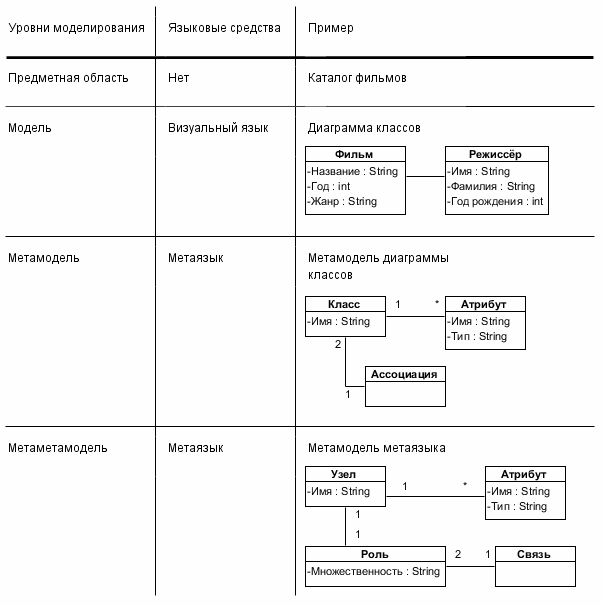
\includegraphics[width=0.9\textwidth]{part1/metalevels.png}
		\caption{Метауровни визуальных языков.}
		\label{metalevels}
	\end{center}
\end{figure}

\textit{Предметная область} --- это то, что мы моделируем, те объекты или явления 
реального мира, с которыми будет работать создаваемое программное обеспечение. 
Предметная область просто существует, и сама по себе никак не описывается, любое 
её описание её упрощает, а значит, будет её моделью. В нашем примере мы хотим 
создать программу --- каталог фильмов, предметная область для такой программы 
будет включать в себя фильмы и всё, что с ними связано --- актёров, режиссёра, 
кассовые сборы, где и когда фильм снимался и т.д. и т.п. Большая часть этой 
информации для наших целей не нужна.

\textit{Модель} --- это некое упрощение предметной области, нужное для выполнения там 
некоторых полезных действий. Предметная область, как правило, обладает 
бесконечным многообразием, и работать со всеми её свойствами невозможно. 
В нашем примере про каталог фильмов нас не интересуют, например, все кинотеатры, 
где показывали фильм, нам интересен только тот ограниченный объём информации,
с которым будет работать создаваемая программа. Для создания модели уже 
используется некий язык. Если это неформальное описание предметной области, в 
качестве языка может выступать естественный язык, если это некая диаграмма, она 
будет рисоваться на некоем визуальном языке. Для нашего примера был использован 
некий сильно упрощённый вариант языка диаграмм классов UML.

\textit{Метамодель} --- это описание визуального языка, то есть множества всех 
синтаксически корректных диаграмм на этом языке, с помощью некоего другого 
визуального языка. Этот язык называется метаязыком, и описывает множество всех 
элементов моделируемого языка и возможные связи между ними. Каждый элемент 
диаграммы на визуальном языке является экземпляром некоторой сущности, описанной 
в метамодели на метаязыке. В нашем примере для моделирования предметной области 
был использован очень простой язык с сущностями "`класс"' и "`атрибут"', и одной 
связью, которая может только связывать два класса и больше никакой информации 
не содержит. Атрибут "`Название"' на диаграмме классов является экземпляром 
сущности "`Атрибут"' в метамодели.

\textit{Метаметамодель} --- это метамодель метаязыка, то есть визуальная модель, 
которая задаёт множество допустимых метамоделей. Имея такую формализацию 
метаязыка, можно создавать инструменты, которые позволяют разрабатывать 
метамодели для произвольных визуальных языков. Интересно, что термин 
"`метаметаязык"', как язык, который используется для создания метаметамодели, 
не требуется --- метаязык сам по себе является визуальным языком, и поэтому, 
если он достаточно выразителен, может быть использован для создания своей 
собственной метамодели. Такой подход, в частности, применён в стандарте UML 
--- сначала вводится метаязык в терминах самого себя (при этом авторам стандарта 
пришлось приложить некоторые усилия, чтобы избежать круговых зависимостей в 
определении), затем с его помощью описывается метамодель UML. В нашем примере 
метаязык очень прост, состоит из сущностей, называемых в метаметамодели 
"`узлами"', и связей. Связи здесь более сложные, чем в языке, потому что мы 
хотим использовать множественность для задания дополнительных ограничений на 
модели. Например, у класса может быть сколько угодно атрибутов, но у атрибута 
может быть только один класс.

Проводя аналогию с текстовыми языками, модель можно сопоставить программе на 
текстовом языке, метамодель --- описание грамматики языка (например, используя 
форму Бэкуса-Наура), метаметамодель --- описание синтаксиса формализма, 
используемого для описания грамматики (например, описание синтаксиса форм 
Бэкуса-Наура, которое тоже можно выполнить с помощью форм Бэкуса-Наура). 
Заметим, что метаязыков может быть много, ведь синтаксис текстовых языков может 
быть описан с помощью различных формальных систем, например, с помощью различных 
языков описания синтаксиса генераторов синтаксических анализаторов, используемых 
для разработки компилятора этого языка. С визуальными языками ситуация 
аналогична.

\section{Предметно-ориентированное моделирование}
\subsection{Понятие предметно-ориентированного моделирования}
Формализмы для задания синтаксиса визуальных языков позволяют эффективно 
создавать новые визуальные языки. Это оказывается полезно не только 
международным группам, занимающимся стандартизацией широко распространённых 
языков визуального моделирования, но и небольшим группам разработчиков, 
создающим визуальные языки для своих проектов. Оказалось, что иногда создать 
специальный язык и решить на нём поставленную задачу можно проще и эффективнее, 
чем решать задачу на языке общего назначения. Особенно это верно в том случае, 
если имеется набор похожих задач, которые можно решать с помощью одного и того 
же языка. Такой подход получил название \textit{предметно-ориентированное моделирование} 
(\textit{Domain-Specific Modeling, DSM}). Основной принцип данного подхода состоит в том, 
что выбирается достаточно узкая предметная область или даже одна задача, 
конкретно для неё создаётся свой язык (\textit{предметно-ориентированный язык}, или 
\textit{Domain-Specific Language, DSL}), и дальше задачи решаются уже на нём. Поскольку 
предметная область узка, то средства инструментальной поддержки созданного языка 
могут использовать знания о предметной области, что позволяет, в частности, 
добиться полной кодогенерации. Кроме того,разработчики, использующие язык, 
работают в терминах, максимально приближенных к предметной области, так что 
программы получаются простыми и понятными даже людям, далёким от 
программирования.

Получаемые благодаря применению этого принципа преимущества по сравнению с 
использованием языков общего назначения таковы.
\begin{itemize}
	\item Программирование ведётся в терминах предметной области, вся рутинная 
		работа выполняется инструментальными средствами, что значительно повышает 
		эффективность труда разработчиков.
	\item Узость выбранной предметной области позволяет обеспечить полную 
		генерацию кода по описаниям на предметно-ориентированном языке. Генератор 
		обладает знаниями о предметной области и использует их, чтобы преодолеть 
		семантический разрыв --- сама программа остаётся простой, генератор тоже 
		может быть устроен довольно просто, но всё вместе позволяет сгенерировать 
		любую нужную программу.
	\item Наличие полной кодогенерации позволяет разработчикам вообще не работать 
		с кодом. Основным артефактом, с которым ведётся работа, являются модели на 
		предметно-ориентированном языке, разработчики могут даже не догадываться о 
		том, что их программы генерируются в код на текстовом языке. Иногда 
		предметно-ориентированное решение устроено так, что генерация в текстовый 
		язык и не требуется (например, модели интерпретируются).
	\item Полная кодогенерация позволяет избежать ошибок кодирования, единственным 
		источником синтаксических ошибок в сгенерированном коде могут быть ошибки в 
		генераторе. При этом исправления и улучшения генератора будут автоматически 
		применимы ко всем программам, его использующим. Кроме того, поскольку 
		инструментальные средства "`знают"' про предметную область, возможно 
		создание верификаторов, проверяющих и семантические ошибки в моделях прямо 
		в процессе моделирования.
\end{itemize}

Естественным образом получается разделение труда между специалистами, 
создающими инструментальные средства и специалистами, их использующими. 
Первая группа должна состоять из весьма квалифицированных специалистов, но 
весьма небольшого их числа, поскольку создать инструментальные средства 
требуется лишь единожды. Вторая группа может состоять из людей, даже вообще не 
владеющих программированием, и их обычно оказывается гораздо больше, чем 
разработчиков инструментальных средств. Поскольку предметно-ориентированный язык 
работает в терминах, близких к предметной области, программирование на нём могут 
осуществлять даже конечные пользователи.

Всё это, по ряду оценок
%TODO CRITICAL:, приведённых в [ссылки на три статьи о повышении производительности труда], 
увеличивает эффективность труда разработчиков от трёх до десяти раз, поэтому 
предметно-ориентированное моделирование --- интересная область для исследований.

Существуют широко распространённые текстовые предметно-ориентированные языки, 
успех которых подтверждает сделанные в этом разделе заявления. Самый известный 
пример --- язык запросов к базам данных SQL. Предметная область этого языка 
ограничивается работой с СУБД, она достаточно узка, чтобы пользователь мог 
работать в терминах, очень напоминающих естественный язык, и при этом все 
необходимые действия, которые было бы весьма сложно описывать на языке общего 
назначения, выполняются самой СУБД. Пользователи языка SQL вполне могут не уметь 
программировать на текстовых языках общего назначения, таких как Java и С\#. 

Второй пример семейства предметно-ориентированных языков --- языки описания 
синтаксически управляемых трансляций для различных генераторов синтаксических 
анализаторов (таких как yacc и его многочисленные варианты, ANTLR
%TODO CRITICAL: [ссылки]
). Программа там пишется в форме, очень похожей на описание контекстно-свободной 
грамматики в форме Бэкуса-Наура, по ней генерируется либо магазинный 
преобразователь, транслирующий созданный язык, либо преобразователь, работающий 
по алгоритму рекурсивного спуска. Генераторы синтаксических анализаторов знают 
достаточно о предметной области, чтобы по простому описанию грамматики языка 
сгенерировать довольно сложный синтаксический анализатор, тогда как ручное его 
кодирование было бы очень сложной задачей (автомат, разбирающий какой-либо 
типичный использумый в промышленности язык программирования, может иметь сотни 
состояний). Наличие таких инструментов делает возможным быстрое создание 
предметно-ориентированных текстовых языков, поэтому генераторы синтаксических 
анализаторов для текстовых языков аналогичны метаредакторам для языков 
графических.

Приведём пример графического предметно-ориентированного языка 
%TODO CRITICAL: из [ссылка на статью Келли]
. Программа на этом языке представлена на рисунке~\ref{dslExample}

\begin{figure} [ht]
	\begin{center}
		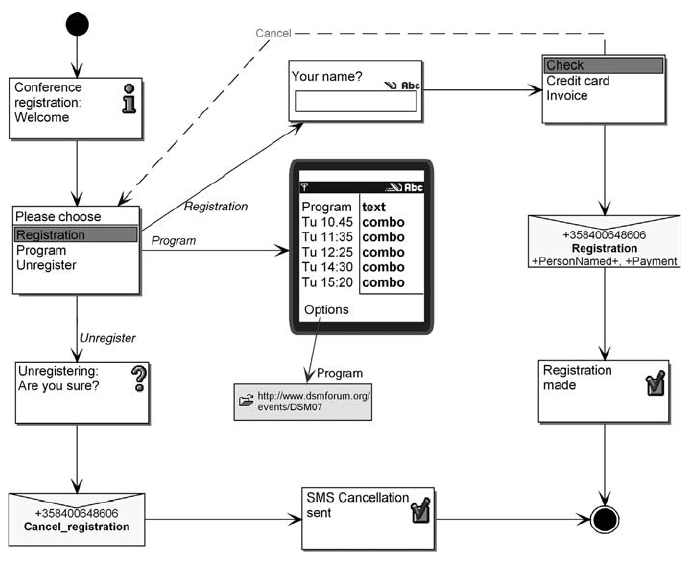
\includegraphics[width=0.9\textwidth]{part1/dslExample.png}
		%TODO: Вставить ссылку на статью Келли вместо Книжки.
		\caption{Пример визуального предметно-ориентированного языка (рисунок из\cite{kelly2008domain})}
		\label{dslExample}
	\end{center}
\end{figure}

Язык предназначается для создания приложений для мобильных телефонов. 
Элементы языка --- это экранные формы, отображаемые на телефоне, связи, 
показывающие порядок перехода между формами, и различные действия, например, 
посылка SMS-сообщения или открытие веб-страницы. На рисунке представлен пример 
программы на этом языке --- программа для регистрации на конференции. 
Как видно, язык достаточно прост и интуитивно понятен, настолько, что не требует 
подробного описания, чтобы читать диаграммы на нём. Вместе с тем, на такой 
диаграмме содержится вся необходимая информация для генерации мобильного 
приложения.
% TODO: прочитать статью и написать поподробнее

\subsection{Инструментальные средства предметно-ориентированного моделирования}
Визуальный предметно-ориентированный язык, или набор языков, и средства 
инструментальной поддержки, такие как редакторы диаграмм, генераторы кода, 
верификаторы, репозиторий, и т.д., всё, что составляет целостную технологию 
разработки программного обеспечения на основе предметно-ориентированного 
подхода, будем называть \textit{предметно-ориентированным решением}, или \textit{DSM-решением}. 
Основные составляющие предметно-ориентированного решения таковы.

\begin{enumerate}
	\item Предметно-ориентированный язык, отражающий специфику предметной области.
	\item Генераторы, извлекающие информацию из модели и формирующие по ней код, 
		документацию, отчёты и т.д.
	\item Предметно-ориентированная библиотека поддержки времени выполнения 
		(domain-specific framework), в которую выносится код, общий для всех 
		программ, создаваемых с помощью DSM-решения. Она служит промежуточным звеном 
		между сгенерированным кодом и целевой платформой, упрощая генератор и убирая 
		дублирование кода в программах. Иногда бывает, что такая библиотека не 
		нужна, генератор генерирует код прямо в целевую платформу, иногда бывает 
		наоборот, библиотека представляет собой по сути движок, интерпретирующий 
		сгенерированные файлы или даже просто конфигурируемый генератором 
		%TODO CRITICAL: (пример такого подхода см., например, в [Сухов-Лядова]). 
		Возможны и промежуточные варианты.
\end{enumerate}

Разумеется, создавать предметно-ориентированные решения вручную было бы слишком 
затратно. Один только хороший визуальный редактор вручную разрабатывается 
несколько десятков человеколет
\footnote{см, например, оценки подобных проектов на ресурсе Ohloh: 
URL: http://www.ohloh.net/p/dia, http://www.ohloh.net/p/umbrello (дата обращения: 14.02.2014)}
, что делает невозможным исполнение главного 
принципа предметно-ориентированного моделирования --- создание языка и всех 
нужных инструментальных средств к нему практически под каждую конкретную задачу. 
Поэтому существуют средства, предназначены для автоматизации разработки 
DSM-решений, их мы, следуя Д. Кознову 
%TODO CRITICAL: [ссылка на релевантные статьи Кознова]
, будем называть \textit{DSM-платформами}. Типичная DSM-платформа позволяет 
специфицировать метамодель языка в текстовом или графическом виде, задать 
внешний вид элементов языка (конкретный синтаксис) и сгенерировать визуальный 
редактор по этим спецификациям. Создание языка обычно требует усилий объёмом 
порядка единиц человекодней или даже человекочасов, что делает возможным 
применение предметно-ориентированного подхода даже в сравнительно небольших 
проектах. Многие DSM-платформы помимо визуального редактора позволяют 
сгенерировать генераторы, верификаторы и другие инструменты, для этого помимо 
метамодели для языка могут быть описаны правила генерации, набор ограничений 
и т.д.

\section{Свойства визуальных языков}
Визуальные языки обладают рядом свойств, некоторые из которых могут быть базисом 
для классификации языков, некоторые важны для реализации некоторой 
функциональности CASE-пакетов и DSM-решений, поэтому вводятся в этом разделе.

Наиболее важное с точки зрения реализации инструментов свойство языков --- 
используемая в них модель представления информации. Предметно-ориентированные 
языки делятся на две крупные категории --- \textit{текстовые} и \textit{графические} 
(или \textit{визуальные}). В данной работе далее будут рассматриваться только визуальные 
языки. 
%TODO: Почему?
Про текстовые языки следует отметить, что не всегда в качестве представления для языков, 
попадающих в эту категорию, используется обычный текст. Возможно использование таблиц, 
возможно древовидное представление структуры программы, и несмотря на то, что программа 
выглядит как текст, для её редактирования требуется специальный редактор (см., например, среду 
JetBrains MPS 
%TODO CRITICAL: [ссылка на MPS]
). Бывает так, что для задания текстовых языков используются визуальные метамодели,
как, например, в~\cite{karlsch2007model}, такие случаи также выходят за границы этого исследования.

Графические языки делятся дополнительно на \textit{графовые} и \textit{неграфовые}. Диаграмма на 
графовом языке представляет собой помеченный мультиграф, либо сводится к нему, то 
есть состоит из множества вершин и множества рёбер, которые их соединяют. 
%TODO: Где-то здесь ссылка на диссер Сухова
Каждая вершина или ребро может обладать различными свойствами, в том числе иметь 
тип, и, соответственно своему типу, отображаться по-разному. Соответственно,
 редакторы таких языков работают в терминах вершин графа (называемых также 
\textit{узлами} или \textit{блоками}) и рёбер (называемых также \textit{связями}). Неграфовые языки --- 
языки, диаграммы на которых не обладают таким свойством. Наиболее распространены 
графовые языки, поскольку редакторы и генераторы для них обычно проще и, 
поскольку логика работы с графовыми моделями не сильно меняется от языка к 
языку, их реализация может быть переиспользована для других языков (что особенно 
важно при разработке DSM-платформ). Для каждого неграфового языка приходится 
обычно писать свой редактор вручную, поскольку такие языки могут быть довольно 
специфичны. Примерами графовых языков могут служить диаграммы классов и 
диаграммы активностей UML, примерами неграфовых языков --- диаграммы 
последовательностей UML (и очень похожий на них язык MSC
%TODO CRITICAL: [ссылка]
), временные диаграммы UML, диаграммы Насси-Шнейдермана
%TODO CRITICAL: [ссылка]
. Данная диссертация посвящена разработке визуальных языков с помощью 
DSM-платформ, на которых графовые языки создавать гораздо удобнее, поэтому 
неграфовые языки, несмотря на то, что довольно распространены и полезны на 
практике, выходят за рамки данного исследования. Многие из результатов, 
описанных в данной работе могут быть без изменений распространены на неграфовые 
языки, но основной фокус в процессе исследования был сделан на графовых языках, 
и апробация результатов проводилась на них.

Существуют и широко распространены языки, комбинирующие свойства текстовых и 
графических --- визуальные языки, которые внутри визуальных символов позволяют 
писать код на текстовом языке, эти языки мы будем называть \textit{текстографическими} или \textit{гибридными}. 
Такой подход с одной стороны совмещает наглядность визуальных языков и лаконичность текстовых языков, с другой стороны 
требует от пользователя знания и визуального языка, и текстовой части, при этом 
текстовая и визуальная части синтаксиса плохо интегрируются (возникает ряд 
проблем, связанных с визуализацией текстовой информации, наличие текстовых
вставок может радикально снижать наглядность). Обычно в качестве текстовых 
вставок используется целевой язык генератора кода по диаграммам, примером такого 
подхода может служить разработанная на кафедре технология RTST 
%TODO CRITICAL: ссылка
. С точки зрения данной работы текст может рассматриваться как свойство элемента 
языка, таким образом, такие языки могут успешно разрабатываться с использованием 
предлагаемой технологии.

Следующее важное свойство языков --- используемая в них модель вычислений. Языки 
делятся по этому признаку опять-таки на две крупные категории --- \textit{статические} 
и \textit{динамические}. 
%TODO: Правда?
Статические языки служат для задания структуры разрабатываемой 
системы, а динамические языки служат для задания поведения системы. Примером 
статического языка может служить диаграмма классов UML или ER-диаграмма, 
описывающая структуру базы данных, примером динамического языка --- диаграмма 
активностей или диаграмма последовательностей UML. Динамические языки, в свою 
очередь, характеризуются формализмом, используемым для определения их семантики, 
поскольку для них применимо собственно понятие "`вычисление"'. Наиболее типично 
применение формализма, являющегося вариантом сетей Петри (граф, по которому 
могут перемещаться токены исполнения
%TODO CRITICAL: Ссылка
), либо диаграмм состояний
%TODO CRITICAL: Ссылка
(наиболее известный вариант которых --- диаграммы Харела 
%TODO CRITICAL: Ссылка
, используемые в языке UML). 

Языки, использующие формализмы, сводящиеся к сетям Петри, имеют две важные с 
практической точки зрения подкатегории. Первая подкатегория языков в качестве 
токенов использует данные, которые обрабатываются программой. Каждый узел языка 
исполняется, когда имеет на всех своих входах данные, нужные ему для работы, 
и результатом его исполнения является набор данных, которые рассылаются на 
выходы блока. Блоки, одновременно имеющие все данные, могут исполняться 
параллельно. Такие языки мы будем называть \textit{языками с процессом вычислений, 
ориентированным на поток данных}. Такие языки широко распространены среди 
инженеров и математиков, примерами сред, реализующих такой подход, являются 
среда математических рассчётов Matlab/Simulink
%TODO CRITICAL: Ссылка
 и среда моделирования физических 
приборов LabView
%TODO CRITICAL: Ссылка
. Вторая подкатегория языков в качестве токенов использует 
нетипизированные токены без дополнительных свойств, характеризующие только 
передачу управления между узлами. Данные при таком подходе не покрываются 
формализмом, описывающим семантику языка, и если всё-таки требуются для работы 
узла, то его поведение может быть не определено, если нужные данные недоступны. 
Параллельное исполнение в таких языках моделируется явно, порождением нескольких 
токенов. Такие языки мы будем называть \textit{языками с процессом вычислений, 
ориентированным на поток управления}. Эти языки широко распространены в 
программной инженерии, примеры --- диаграмма активностей UML и обычные 
блок-схемы.

Далее введём свойства, специфичные для данной работы. Первое такое свойство 
--- поддержка языком переиспользования своих конструкций. В распространённых 
текстовых языках переиспользование занимает одну из центральных ролей, и 
реализуется разными способами --- выделением общих фрагментов кода в макросы 
препроцессора, в функции или процедуры, в шаблоны или генерики и т.д., 
системы типов объектно-ориентированных языков также ориентированы на 
переиспользование. В визуальных языках реализации возможности переиспользования 
обычно уделяют меньше внимания. Не все виды переиспользования реализуемы во всех 
языках, например, в статических языках типа диаграммы классов UML трудно 
придумать аналогию выделения общего кода в функцию. Первый рассматриваемый 
здесь вид переиспользования --- \textit{переиспользование копированием} 
%TODO: перечитать курсовую Нефёдова и написать аккуратнее
%TODO: убедиться, что это обсуждается в разделах дальше (про эксплозии и в апробации)
--- реализуем 
во всех языках. Заключается он в том, что фрагменты моделей, которые требуется 
использовать повторно, просто копируются в то место, где они нужны. Это полный 
аналог операции "`copy and paste"' в текстовых языках и имеет те же недостатки 
--- при изменении одного фрагмента все его копии требуется обновлять вручную, 
растёт объём кода. \textit{Переиспользование вызовом} требует от визуального языка 
понятий "`подпрограмма"' и "`вызов подпрограммы"', или их аналогов, что, в свою 
очередь требует наличия у языка семантики вычислений, и, таким образом, 
применимо только к динамическим языкам. Этот вид переиспользования --- аналог 
использования функций в текстовых языках: общий фрагмент моделей выносится в 
отдельную сущность (отдельную диаграмму, контейнер, что-то ещё), после чего во 
все места, где этот фрагмент требуется, добавляется элемент "`вызов"' со 
ссылкой на вынесенный фрагмент. Несмотря на большое количество условий, 
накладываемых на язык, этот вид переиспользования активно применяется на 
практике.
%TODO: Где?
 \textit{Переиспользование по интерфейсу} является неким обобщением 
переиспользования по вызову и применимо для статических языков, где нет понятия 
"`вызов"'. Фрагмент модели, который требуется переиспользовать, выделяется в 
отдельную сущность, для этой сущности создаётся элемент, который 
"`представляет"' эту сущность в тех местах, где необходимо переиспользовать 
фрагмент. Такой метод переиспользования аналогичен переиспользованию классов 
или фасадов подсистем или компонент в текстовых языках --- для подсистемы 
создаётся некий интерфейс, по которому её функциональность вызывается в тех 
местах системы, где она требуется. Этот метод требует поддержки в семантике 
языка, поскольку только сам язык может содержать информацию о том, как 
интерпретировать свойства сущности-представителя и что для неё 
"`переиспользование"'. Пример такого способа переиспользования --- в языке 
диаграммы классов UML можно описать подсистему, описать для неё интерфейс и 
использовать этот интерфейс на других диаграммах. При этом интерпретация такой 
ситуации как переиспользования фрагмента диаграммы, скорее всего, будет 
ответственностью пользователя языка, либо же графический редактор должен иметь 
поддержку такого способа переиспользования конкретно для диаграммы классов UML 
(например, рефакторинг "`выделить в отдельную диаграмму"'). Отметим, что с 
точки зрения автоматизации разработки редактора языка этот способ 
переиспользования представляет наибольшую сложность --- если переиспользование 
копированием можно реализовать языконезависимо, а переиспользование вызовом --- 
введением возможности описания семантики вызова в метаязык, то 
переиспользование по интерфейсу как правило оказывается слишком специфично для 
конкретного языка.

Следующее свойство визуальных языков, отчасти связанное с переиспользованием 
--- существенность для семантики языка того, как именно выглядят диаграммы. 
Для пояснения этого потребуются ещё два понятия --- логическая и графическая 
модели. 
%TODO: Это бред какой-то, нужно обсудить и написать аккуратнее
\textit{Логическая модель} --- часть модели системы, которая существенна для 
функционирования системы, графическая модель --- часть модели, которая имеет 
значение для представления модели пользователю в процессе разработки системы. 
То есть, логическая модель --- это то, что важно для генератора, графическая 
модель --- то, что видит пользователь. Соответственно, свойства сущностей языка, 
которые относятся к логической модели (важны для генератора) назовём \textit{логическими 
свойствами}, свойства, относящиеся к графической модели --- \textit{графическими 
свойствами}. Назовём \textit{существенно графическими языками} языки, в которых 
графическая модель оказывает существенное влияние на функционирование системы, 
то есть внешний вид диаграмм, геометрическое расположение на них элементов 
и т.д. оказывают влияние на их семантику (например, на результат работы генератора). \textit{Языками с выделенной 
логической моделью} будем называть языки, для которых это не так. Для таких 
языков диаграммы как правило являются лишь средством редактирования логической 
модели, и логическая модель может существовать вообще независимо от 
представления. Пример существенно графического языка --- временная диаграмма 
UML, там временные интервалы определяются длиной линий. Пример языка с 
выделенной логической моделью --- язык диаграммы классов UML, модель классов 
системы может быть произвольно разбита на диаграммы, классы на диаграмме могут 
располагаться произвольным образом, важны только их свойства и то, с какими 
элементами они связаны (при этом, расположение связей и даже то, изображены 
они на диаграмме или нет, не имеет значения). Графовые языки обычно имеют 
выделенную логическую модель, неграфовые языки имеют тенденцию быть существенно 
графическими, однако бывают исключения. Например, автором данной работы был 
реализован язык описания конечного автомата, распознающего жесты рукой для 
системы компьютерного стереозрения. Там состояния было удобно связывать с 
физическим расположением руки в пространстве, и от геометрического расположения 
на диаграмме элементов языка зависела генерация правил перехода. Язык был 
графовым (узлами были состояния автомата, связями --- переходы), но при этом 
существенно графическим.

С переиспользованием разделение на логическую и графическую модель языка связано 
следующим образом --- языки с выделенной логической моделью позволяют 
использовать один и тот же элемент логической модели на разных диаграммах или 
в разных местах одной диаграммы. Если редактор для этого языка позволяет, можно 
редактировать логические свойства элемента у любого из его графических 
"`образов"', и все остальные "`образы"' получат эти изменения автоматически. 
Такой способ переиспользования является подвидом переиспользования 
копированием, но инструментальные средства берут на себя поддержание 
консистентности модели при изменениях. 
%TODO: неплохо бы единый фреймворк для классификации языков, или хотя бы написать про 
%      статью из курсовой Гудошниковой
